\documentclass[11 pt, a4paper]{article}  % list options between brackets
\usepackage[nottoc,notlof,notlot,numbib]{tocbibind}
\usepackage[margin=1.2 in]{geometry}
\usepackage{fancyhdr}
\usepackage{manfnt}
\usepackage{pgf}
\usepackage{amsmath,amssymb,natbib,graphicx}
\usepackage{amsfonts}
\DeclareMathAlphabet{\mathpzc}{OT1}{pzc}{m}{it}
\usepackage{bbm}
\usepackage{hyperref}
\usepackage{float}
\usepackage{mathrsfs} %mathscr{A}

\usepackage{chngpage}
\usepackage{layouts}

\usepackage{times}
\usepackage{latexsym}
\usepackage{caption}
\usepackage{graphicx}

\usepackage{subcaption}

\usepackage{algorithm}
\usepackage[noend]{algpseudocode}

\newtheorem{axiom}{Axiom}[section]
\newtheorem{result}{Result}[section]
\newtheorem{example}{example}[section]
\newtheorem{definition}{Definition}[section]
\newtheorem{principle}{Principle}[section]
\newtheorem{theorem}{Theorem}[section]% list packages between braces

% type user-defined commands here
%\newcommand{\vmu}{{\bf \mu}}
%\newcommand{\vtheta1}{{\bf \theta^{(1)}}}
%\newcommand{\vtheta2}{{\bf \theta^{(2)}}}
%\newcommand{\vpi}{{\bf \pi}}}

\newcommand{\gm}{\gamma}


\linespread{1.3}
\begin{document}

\title{Bayesian latent class model with sparse correlation for etiology estimation}   % type title between braces
\author{Detian Deng}         % type author(s) between braces
\date{\today}    % type date between braces
\maketitle

%\begin{abstract}
%\end{abstract}
\section{Introduction}
\subsection{Background}
\subsubsection{Child Pneumonia}
Pneumonia is a form of acute respiratory infection of the lungs\cite{WHO}. The infection can be caused by a variety of pathogens, indcluding bacteria, viruses, mycobacteria and fungi \cite{hirama2011prediction}. When a child under five gets pneumonia, the typical symptoms may include fever, cough, fast or difficult breathing, lower chest wall indrawing where the chest moves in or retracts during inhalation, and wheezing \cite{singh2011pneumonia, WHO}. Severe cases may be unable to feed or drink and may also experience unconsciousness, hypothermia and convulsions \cite{WHO}. Although the majority of child pneumonia cases are nonsevere and can be managed in local primary health care facilities \cite{levine2012pneumonia}, the severe/very severe cases may result in death, especially in developing countries. In fact, pneumonia is the single largest infectious cause of death of children under $5$ years of age (referred to ``children'' for the rest part of this article) , with an estimate of $1.6$ million deaths per year accounting for $18\%$ of the total $8.8$ million childhood deaths worldwide \cite{liu2012global, black2010global}. Under the pressure of such a severe public health burden, UNICEF and WHO declared pneumonia to be the ``forgotten killer of children'' in 2006 \cite{unicef2006pneumonia} and engaged the Global Action Plan for Prevention and Control of Pneumonia (GAPP) \cite{world2009global} in 2009. \\


\subsubsection{The Need of New Etiology Information}
Current prevention and treatment strategies for pneumonia were primarily developed based on the results of early pneumonia etiology studies in the 1980s \cite{shann1986etiology, world1990programme}, in which two bacterial pathogens, streptococcus pneumoniae and haemophilus influenzae, were identified as the primary etiologies of pneumonia mortality. It has been 30 years since those studies conducted, and by 2015, three major changes will have taken place \cite{levine2012pneumonia}: the wide use of pneumococcoal and haemophilus influenzae-B conjugate vaccines; the wide spread of HIV infection \cite{calder2009evidence}; the substantial improvements/changes in living conditions, nutrition, and access to health care. These changes will certainly modify the distribution of pathogens, the transmission, and the natural history of infection, which will make the understandings of pneumonia etiology based on the early studies invalid. Hence the effectiveness of the current prevention and treatment could be greatly diminished. \\

As a result, new information of the current etiology of severe/very severe pneumonia for children under 5 is required to ensure its prevention and treatment strategies are appropriate and effective for the epidemiologic setting of the future. In the context of such a strong need, the Pneumonia Etiology Rearch for Child Health (PERCH) project, the largest of its kind in over 20 years, was launched in 2011 and finished data collection recently.\\

% Accurate estimate of its etiology will directly lead to improvement in prevention strategies and therapies for such a deadly disease for children.

\subsubsection{Pneumonia Etiology Rearch for Child Health}
The PERCH project is a case-control study that enrolled around 9500 children from 7 sites across the globe with the primary goals \cite{levine2012pneumonia} to: 
\begin{itemize}
\item Estimate the association between severe/very severe pneumonia and infection with confirmed and putative viral, bacterial, mycobacterial, and fungal pathogens.
\item Learn the probability of severe/very severe pneumonia attributable to each of the candidate pathogens.
\item Evaluate potential risk factors for infection and/or severe/very severe pneumonia due to novel or under-recognized etiologic pathogens. 
\end{itemize} 

A case-control design was chosen because it is more efficient than cohort studies and probe studies in terms of identifying the etiology among many different, putative etiologic pathogens. The 7 study sites are in Bangladesh, Gambia, Kenya, Mali, South Africa, Thailand and Zambia. These sites were chosen to represent the developing countries with major childhood pneumonia burdens and a range of diverse epidemiologic settings. The study enrolled about 4200 children hospitalized for severe/very severe pneumonia and approximately 5300 controls randomly selected from the corresponding communities. The inclusion-exclusion criterion are discussed in detail by Deloria-Knoll et al.\cite{deloria2012identification}. For each enrolled subject, data on demographics, known and putative risk factors, and pathogen infection were collected. \\

More explanation on the rationale of the study can be found in the review by Adegbola, RA and Levine, OS \cite{adegbola2011rationale}. 

\subsubsection*{Specimen Measurements and Data Description}
In order to maximize the detection power and accuracy of pathogen infection, the PERCH investors used multiple specimen types \cite{hammitt2012specimen} including acute blood (for cases only), nasopharyngeal(NP) swab (for both cases and controls), and lung aspirates (for only very few cases). These samples were collected and tested by a variety of conventional and novel detection techniques such as microscopy, culture, serology, antigen testing, and polymerase chain reaction (PCR) \cite{murdoch2012laboratory}, targeting on more than $30$ candidate pathogens. An example of a single test record is shown in table \ref{test_eg}. 
\begin{table}[h]
\centering
\caption{Test record indicates that Haemophilus influenzae is detected by PCR in the lung aspirate specimen of subject 1.}
\label{test_eg}
\begin{tabular}{llllll}
\hline
subject ID & Group & Specimen Type & Detection Technique & Pathogen Name          & Test Result \\ \hline
1          & Case  & Lung aspirate & PCR                 & Haemophilus influenzae & positive           \\ \hline
\end{tabular}
\end{table}

Tests based on lung aspirates samples are considered to provide the direct observation of the lung and are assumed to have perfect sensitivity and specificity, thus they are called Gold Standard (GS) measurements. Among all peripheral measurements, we assume blood samples provide measurements with perfect specificity, but imperfect sensitivity, and NP samples provide both imperfect sensitivity and specificity, thus we call measurements from blood samples Silver Standard (SS) measurements, and those from NP samples Bronze Standard (BS) measurements.\\

For each child (patient) $i$, let $Y_i$ indicate whether this child is a case ($Y_i=1$) or a control ($Y_i=0$). Suppose there are $K$ pre-specified pneumonia causing candidates, the list of measurements can be described by three $K$-dimensional binary vector: $M_i^{GS}$ (if available), $M_i^{SS}$, and $M_i^{BS}$, where $M_{ik}^{Src}=1$ indicates that the $k$th pathogen is detected using the $Src \in \{GS, SS, BS\}$ measurements in subject $i$. The data availability and the format of measurement vector are summarized in Figure \ref{data}. \\

\begin{center}
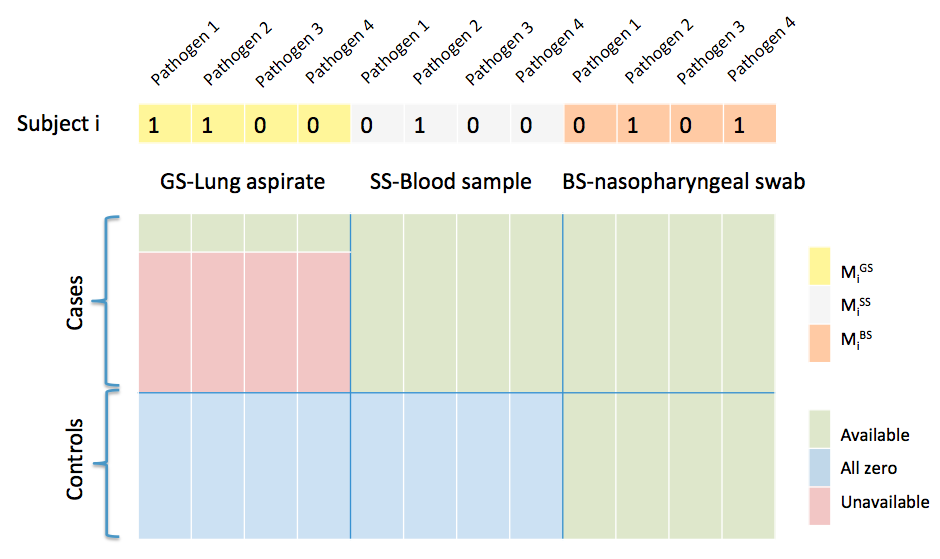
\includegraphics[scale=0.45]{DataDescription.png}
\captionof{figure}{{\bf Data Description}: Suppose we have 4 candidate pathogens in this demonstrative example. In the upper part of this figure, the three 4 dimensional vectors $M_i^{GS}$, $M_i^{SS}$, and $M_i^{BS}$ are concatenated together. The GS measurement is available and it tells us pathogen 1 and 2 infect the lung of subject $i$. Due to the imperfect sensitivity, SS and BS measurements fail to detect pathogen 1. And because of the imperfect specificity, BS measurement detects a false positive for pathogen 4. In the lower part of this figure, the data availability is represented by different colors. As we can see, only a small fraction of cases have GS measurements.}
\label{data}
\end{center}

\subsection{Statistical Framework and Challenges}
Due to the invasiveness of the lung aspirate procedure, GS measurements were rarely acquired \cite{levine2012pneumonia, hammitt2012specimen}. The actual pathogen(s) that infect the lung therefore can only be inferred from multiple peripheral measurements with imperfect sensitivity and/or specificity, i.e. the actual lung infection is a latent variable for cases. This fact poses significant statistical challenges for estimating the prevalence of the etiologic pathogens in the population of children, especially in the situation where there are multiple pathogens infecting the lung.In machine learning terms, the problem is ``unsupervised'' absent the GS data \cite{friedman2001elements}.\\

Let $L_i$ be a $K$-dimensional binary vector describing the latent lung infection status for child $i$, where $L_{ik}=1$ indicates the child's lung is infected by the $k$th pathogen. $L_i = (0,\ldots,0)^T$ means the child has no infection in his/her lung, which is believed to be the true lung status for each control. We also assume, with small probability $\pi_0$, a patient identified as case has no infection in his/her lung: $L_i = (0,\ldots,0)^T$. Using notations defined so far, our interest in this thesis project can be formulated as to estimate the population mean of true lung status of child pneumonia cases given peripheral measurements data, that is, $\mu = \mathbb{E}[L|M^{GS},M^{SS},M^{BS},Y=1]$. We will call this parameter the etiology fraction in the following discussion.\\

Given that most of the measurements are imperfect in terms of sensitivity and specificity, neglecting or inappropriately adjusting (e.g. guessing the wrong value of sensitivity/specificity) for measurement error can produce significantly biased estimates \cite{gustafson2002bayesian}. Therefore, developing a statistical method for estimating $\mu$ that appropriately adjusts the measurement errors and incorporates all available sources of evidence is crucial to achieving the goal of PERCH. \\

Recently, Wu, et al. (2015) developed the partially-Latent Class Model (pLCM)\cite{wu2015partially} and the nested-pLCM (npLCM) \cite{wu2015nested}, introduced in the next section, as extensions to the classic Laten Class Model \cite{goodman1974exploratory}, in order to deal with issues mentioned above. In this thesis project, we propose to further extend the pLCM framework in three ways. First, pLCM and npLCM assumes that a only one pathogen can be the true cause of disease for a case subject, but scientists often argue that there is a non-negligible probability that two or more pathogens can jointly cause pneumonia for a child. Our extension will allow for multiple pathogens to constitute the sufficient cause\cite{rothman2008modern}. Second, in pLCM, the pneumonia case definition is assumed to be error free. In our model, we will allow for misclassification of cases and controls. Third, an novel prior specification is introduced to facilitate better incorporation of scientific knowledge. Specifically, we will place informative prior information on both the chance that each pathogen is part of the sufficient cause and on the number of pathogens that constitute the sufficient cause. We will study whether these three changes provide a better approximation to the true disease-causing mechanism and will yield more accurate estimates of the parameter of interest.\\

In section 2, models for multivariate binary data and the latest developments on partial latent class models are reviewed. In section 3, the redesigned representation of $L$ is described. And in section 4, the full specification of our proposed model is explained. The future work is discussed in section 5. The model fitting algorithm is presented in the appendix.
 
\newpage
\section{Literature Review on Related Statistical Methodologies}
In the previous section, we have identified the challenging statistical problem posed by the PERCH study, essential to the prevention and treatment of childhood pneumonia. In this section, we will review the current statistical methods that are relevant to solving this type of problem, introduce the foundations on which our method is based, and briefly explain what advantages our model should achieve.

\subsection{Partially-Latent Class Model and Nested Partially-Latent Class Model}
Latent class model (LCM) \cite{goodman1974exploratory} is a statistical model for identifying unobserved subgroups of the population from multivariate categorical data. The model is parameterized by the prevalence of each latent class and the the conditional probabilities for the observed data given each class membership. Traditionally, given the latent class membership, the observed data are assumed to be conditionally independent. This type of model has a wide range of applications\cite{rindskopf2002use, albert2001latent}, in which we will focus on the use in estimating the etiology fraction given multiple indirect measurements.\\

In this application, however, the classical LCM has its limitations. First, in the classical LCM, the number of latent classes is determined by comparing the goodness-of-fit of different models, thus the latent classes identified do not always have clear interpretations. Second, the classical LCM cannot use the partly available gold standard data and the control data. Third, it suffers from weak model identifiability \cite{goodman1974exploratory} when the number of latent categories are large.\\

Therefore, Zhenke Wu, et al.(2015) developed the Bayesian partially-Latent Class Model (pLCM) \cite{wu2015partially} to estimate the population etiology distribution using PERCH data. In this model, the latent classes are specifically defined as the true infection of the lung. The conditional distributions of the measurements given the true infection are characterized by sensitivities and specificities. Then the marginal likelihood of the multivariate measurements is modeled as a function of the etiology fraction, sensitivities and specificities. This model also makes use of both control and GS, SS, and BS data. Absent GS data, the model is only partially identifiable \cite{jones2010identifiability} as termed in Jones et al.(2010). That is, to estimate the etiology fraction, prior information about the measurement sensitivities is needed. Specificities can be estimated from the control data. Furthermore, Wu, et al. extends pLCM to the nested-pLCM \cite{wu2015nested} by building sub-classes nested under the latent disease classes to allow dependency among measurements given the latent class.\\

It is important to note that the pLCM and the npLCM were both built on the assumption that each case has a single cause infecting the lung, where this cause can be a single pathogen from the list of candidates or a pre-fixed combination of candidate pathogens. This single-cause assumption enables the model to use the multinomial stochastic framework, i.e. the latent lung status is assumed to be a multinomial variable $I_i$ with $\omega_k=P(I_i=k)$ and $\sum_{k=1}^K \omega_k=1$, where $\omega_k$ is the fraction of of disease caused by the $k$th pathogen or pathogen combination. This framework is conceptually straightforward and computationally efficient, because the marginal likelihood has the simple form of $\prod_i \sum_k \omega_k P(M_{i}|I_i=k,\lambda)$ where $\lambda$ includes the sensitivities and specificities. By choosing appropriate conjugate priors for $\{\omega_k\}_{k=1}^K$ and $\lambda$, an efficient Gibbs Sampling algorithm can be derived. \\

However, the single-cause assumption is often questioned by physicians and scientists, since indirect measurements in previous studies \cite{cilla2008viruses, toikka2000streptococcus} suggested possible bacterial and viral coninfections for pneumonia cases and bacterial coinfections in lung tissue specimens were confirmed in the study of 2009 pandemic influenza A (H1N1) \cite{louie2009bacterial}. If pathogen coinfections for pneumonia were frequent, the etiology fraction $\omega_k$ would be biased and tend to be smaller since the sum of the true probability of pneumonia attributable to each of the candidate pathogens would be greater than one. \\

Therefore, we propose to develop a model that allows multiple pathogens to cause the disease without having to specify in advance which subset of combinations is allowed. In order to achieve this goal, we propose to model the latent status of the lung as a multivariate binary vector $L_i$ as defined in section 1. Next, we will review the current methods for modeling multivariate binary data.\\


\subsection{Models for Multivariate Binary Data}
Multivariate binary data, or multidimensional contingency table, have been extensively studied since the 1960s. A large collections of statistical models have been proposed, and they can be generally categorized into two classes: the likelihood based approach \cite{haberman1973log, fitzmaurice1993likelihood, ekholm1995marginal, zhao1990correlated} and the non-likelihood based approach \cite{liang1986longitudinal, zeger1988models, lipsitz1991generalized}. In this proposal, we focus on the likelihood approach in order to integrate it in the new latent class model.\\

We will briefly review the main methods for parameterizing the multivariate binary distribution in this section, and for each method the important parsimonious extensions and corresponding regression models will also be discussed.\\

\begin{itemize}
\item {\bf Multinomial distribution}: 
Consider a multivariate binary vector of length $K$, denoted by $L=(L_1,\ldots,L_k)$. There are $2^K$ possible observations for $L$, termed cells. Let each cell probability be $P(L=l) = p_l$ with $\sum_l p_l = 1$, then $L$ is a multinomial variable with $2^K -1$ independent parameters. This is the most straightforward and flexible model but has bad scalability since the number of parameters grows exponentially as the dimension grows. Also, it gives little insight into the structure of the data \cite{cox1972analysis}, thus it is hard to find a parsimonious extension of it and few regression models were built upon it.\\


\item {\bf Bahadur representation}: 
First suggested by Bahadur (1961) \cite{bahadur1961representation}  and later by Cox (1972) \cite{cox1972analysis}, this representation models the joint probability of the multivariate binary data as a functions of the marginal probabilities and the second and higher-order correlation. Let $\theta_j = P(L_j=1)$ and standardize the data as $U_j=(L_j-\theta_j)/\sqrt{\theta_j(1-\theta_j)}$. Define $\rho_{12\ldots k}=\mathbb{E}(U_1\ldots U_k)$ as the $k$th order correlation between $L_1,\ldots,L_k$. Then the joint probability is defined as 
\[P(L=l)=\prod_{j=1}^K P(L_j=l_j) \Big \{ 1+ \sum_{i>j}\rho_{ij}u_i u_j +  
\sum_{i>j>k}\rho_{ijk}u_i u_j u_k + \ldots + \rho_{12 \ldots d}u_1\ldots u_d \Big \}\]

This representation is also a saturated model with $2^K -1$ independent parameter. To reduce the number of parameters, one can assume parsimonious models for the correlation structure. For example, one could assume an ``exchangeable'' correlation structure, in which the $k$th-order correlations are all the same. Then the parameters would only increase linearly with the dimension. In the extreme case where all correlation parameters are set to zero, this representation becomes an independence model.\\

Estimation methods for regression models using Bahadur representation were discussed by Lipsitz, et al. (1995) \cite{lipsitz1995estimation}. Since the maximum likelihood (ML) estimation with a Newton-Ralphston algorithm requires very large sample size compared to the dimension to converge to a unique solution, they proposed the ``one-step'' ML estimator and proved that it is asymptotically equivalent to the fully iterated ML estimator. An alternative moment-based estimation approach\cite{lipsitz1995estimation} was also developed as an extension to Liang and Zeger's (1986) generalized estimating equations (GEE)\cite{liang1986longitudinal}.\\

\item {\bf Log-linear Models}: 
The general log-linear model, first described by Cox (1972) \cite{cox1972analysis} and discussed in depth by Haberman (1973) \cite{haberman1973log}, is the most widely used parameterization for multivariate binary data. This representation models the joint probability in the log scale as a linear function of conditional log odds' and conditional log odds ratios. It is a member of the exponential family, thus many useful properties can be directly obtained. The general form of log-linear model can be written as:
\[
P(L=l; \Theta) =  \exp \Big\{\Theta_1^T l + \Theta_2^{T} w_2 + \ldots + \Theta_K^T w_K \Big \} /  A(\Theta)
\]

where $w_k$ is a ${K \choose k} \times 1$ vector of the $k$-way cross-products of $l$, $k = 1,\ldots,K$,  and $\Theta = (\Theta_1,\ldots, \Theta_K)$ contains the the canonical parameters, which is a $(2^K-1) \times 1$ vector. $\Theta_1$ contains the $k$ conditional log odds' and the rest contains the conditional log odds ratios, regarded as the association parameters. Moreover, let $l^* = (l,w_2,\dots,w_K)^T$, the normalizing term is defined as
\begin{align*}
A(\Theta) = & \sum_{l^*:l\in \{0,1\}^K}\exp \{ \Theta^T l^*\} 
\end{align*}

Similar to the Bahadur representation, the above model allows for varying degrees of dependence among $\{ L_j \}_{j=1}^K$. Independence model is achieved when all of the tow- and higher-way association parameters are set to zero. And the other extreme is to use the full $2^K-1$ parameters to form a saturated model. \\

A variety of parsimonious extensions and re-parameterizations have been developed based on the log linear model. An important special case is the ``quadratic expoential family'' described by Zhao and Prentice (1990) \cite{zhao1990correlated}, which fixes the three- and higher-way association parameters at zero. In addition, they made a one-to-one transformation from $(\Theta_1, \Theta_2)$ to the marginal moment parameters $(\mu,\sigma)$, where $\mu$ is the vector marginal mean and $\sigma$ is the vector of pairwise covariances, and they derived the likelihood equation  for estimating the coefficients of the regression models for $\mu$. However, the problem of this method is that the consistency of the regressions parameters requires the correct specification of both the means and pairwise correlations.\\

As a method to circumvent the drawback of the above model, an important re-parameterization of the general log-linear model, the ``mixed parameter''  model, is proposed by Fitzmaurice and Laird (1993) \cite{fitzmaurice1993likelihood}. Let $\Omega = (\Theta_1,\ldots, \Theta_K)$, the model is parameterized in terms of $(\mu, \Omega)$, the mixture of marginal mean and conditional log odds ratios, via the one-to-one transformation from $(\Theta_1, \Omega)$ to $(\mu, \Omega)$. Although such transformation has no closed form, the problem can be solved  using the iterative proportional fitting algorithm (Deming and Stephen, 1940) \cite{deming1940least} within each step of the Fisher scoring algorithm. And it is shown that the regression coefficient estimator is consistent if the mean structure is correctly specified even if the correlation structure $\Omega$ is not.\\

\item {\bf Dependence Ratio Model}:
The dependence ratio model was proposed by Ekholm (1995) \cite{ekholm1995marginal}, which models the association using dependence ratios rather than odds ratios. Let $\eta = (\eta_1, \ldots, \eta_K, \eta_{12}, \ldots, \eta_{1\ldots K}) = \mathbb{E}(l^*)$.  The $k$th-order dependence ratio is defined as the joint success probability of $k$ binary responses divided by the joint success probability assuming independence. For example, the 2nd order dependence ratio between $L_1$ and $L_2$ is $\lambda_{12}=\frac{\eta_{12}}{\eta_1\eta_2}$. Therefore, dependence ratio being one indicates independence. It is shown that the joint probability can be expressed as an affine linear transformation of $\eta$ and a marginal regression model is built. Furthermore, Ekholm (2000) \cite{ekholm2000association} suggested five types of parsimonious association models by constraining the structure of $\eta$ based on this representation.\\


\item {\bf Latent Continuous Distribution}:
A multivariate binary distribution can be obtained from a multivariate continuous distribution by thresholding each of the variables. For example, consider a multivariate Gaussian random vector $Z=(Z_1,\ldots , Z_K)$, the corresponding multivariate binary distribution can be constructed by letting $L_j=1$ if and only if, say, $Z_j>0$ and letting $L_j=0$ other wise. This model, considered by Cox (1972), as a ``historically important way'' and a ``useful heuristic device'' but ``seems unnecessary unless the $Z$'s are of intrinsic interest''.   

\item {\bf Lattice Based Model}
The lattice based models are extensively studied and widely used in the field of spatial analysis and statistical mechanics. The early work can date back to the Ising Model (1925) \cite{ising1925beitrag} and currently there are two dominant approaches for modeling binary data on a lattice: the spatial generalized linear mixed model which models the dependence by latent Gaussian Markov random field over the lattice \cite{banerjee2014hierarchical} and the autologistic model, which models the dependence directly \cite{besag1974spatial} thorough a linear function of the neighboring variable, termed autocovariate. The later approach is of more interest in terms of our likelihood specification, so we will focus on the autologistic model in this section.\\

Suppose the multivariate binary data $L\in \{0,1\}^K$ are placed on a lattice. The conditional distribution of $L_j$ is given by:
\[
P(L_j|L_{-j}) = \text{logit}^{-1} \Big ( \beta_j + \sum_{k\neq j} \alpha_{jk}L_k \Big )
\]
where $\beta_j$ is the conditional log odds, $\{\alpha_{jk}\}$ are the dependence parameters, and the sum is called the autocovariate, which determines the dependence between $L_j$ and all the other variables on the lattice $L_{-j}$. Let $\delta_{jk}$ be the indicator of whether $L_j$ and $L_k$ are neighbors, let $D$ be a $K\times K$ adjacency matrix where $[D]_{jk}=\delta_{jk}$, and assume $\alpha_{jk}=\alpha \delta_{jk}$. By Brook's Lemma, the joint distribution of $L$ is
\begin{align*}
P(L|\beta,\alpha) = \frac{\exp \big ( L^T\beta + \frac{\alpha}{2} L^T D L \big )}
{\sum_{Y\in \{0,1\}^K } \exp \big ( Y^T\beta + \frac{\alpha}{2} Y^T D Y \big )}
\end{align*} 
Thus this model can be also viewed as a special case of the log-linear model.
\end{itemize}


% Although the exact mechanism is not fully understood, scientists believe that due to this competition, there cannot be too many pathogens, say, at most 3, that infect the lung at the same time.

\newpage
\section{Representation of the Multivariate Binary Latent Variable for Multiple Cause Etiology}
In order to allow the possibility of multiple pathogens infecting the lung, a multivariate binary vector $L\in \{0,1 \}^K$ is used as the latent variable that describes the true status of the lung. Among all methods reviewed in the previous section, the log-linear model has the following advantages that are important to the etiology estimation problem. (1) It has all the properties of an exponential family distribution; (2) its association parameters are orthogonal to the first order parameters, thus it is more convenient to do stratified estimation and conditional regression modeling on the etiology parameter $\mu=\mathbb{E}(L|M,Y=1)$ (3) association parameters have intuitive interpretations that reflect the complex interactions among various pathogens. \\

Moreover, what the etiology estimation problem also requires but the classic log-linear model does not have, are good scalability in terms of the sample size as well as the number of candidate pathogens, and of course, good identifiability with low quality measurement data. In addition, in the PERCH study, scientists would like to incorporate their prior knowledge in the model that there exists strong competition among the majority of pathogens when they infect the lung, while other few pathogens might infect independently.\\

Thus, we propose a parsimonious quadratic exponential representation for the latent vector $L$, and extend the Bayesian partially-Latent Class Model (pLCM) accordingly, for more accurate etiology estimation. In the rest of this section, we will re-introduce the log-linear model in the context of PERCH study and derive our method from it.\\


\subsection{Log-Linear Model}
Recall that $L$ is a K-dimensional binary random variable denoting the true state of the lung. With the same notations used in last section, the general form of the log-linear model is:
\begin{align*}
P(L=l; \Theta) = & \exp \{\Theta_1^T l + \Theta_2^{T} u_2 + \ldots + \Theta_K^T u_K\}/ A(\Theta) \\
\text{where }\ 
A(\Theta) = & \sum_{l^* \in \{0,1\}^K}\exp \{ \Theta^T l^*\}
\end{align*}
\\
Furthermore, let $S_i \in \{0,1,\ldots, K\}$ be the total number of pathogens infecting the lung of the $i$th patient, i.e. $S_k=\sum_{k=0}^K L_{ik}$, and define $\pi_s=P(S_i=s)$, thus $\pi=(\pi_0,\ldots,\pi_K)$ are the parameters that reflects the knowledge on how many pathogens there can be in the lung. Let $\mu = (\mu_1, \ldots,\mu_K) = \mathbb{E}(L|M,Y=1)$ denote the parameter of our primary interests, where $\mu_k$ is the fraction of disease potentially caused by the $k$th pathogen\footnote{ It is not possible from observational data to determine whether an infection in the lung is part of the sufficient cause or not. That can only be determined by experimentation. Therefore, we are estimating the pathogens infecting the lung whether they constitute the cause or not.}. Since we allow multiple pathogen infection, the sum of all these fractions may be greater than $1$. By plugging in the above joint probability function, we have
\begin{align}
\pi_s := & P(S=s)\nonumber \\ 
= & \frac{1}{A(\Theta)} \sum_{l^*:S=s}\exp \{ \Theta^T l^*\}  \text{ , } s = 1,\ldots, K \\
\pi_0 = & \frac{1}{A(\Theta)} \nonumber \\
\mu_k = & \frac{1}{A(\Theta)} \sum_{\tilde{l}:l_k=1}\exp \{ \Theta^T l^*\}  \text{ , } k = 1, \ldots, K
\end{align}
\\
Note that $l^*$ has length $2^K-1$, and by stacking all possible values of $l^*$ except for the zero vector together, we get a square matrix $L^*$ with dimension $J = 2^K-1$.
As we can see, it is hard to re-parameterize the log-linear model directly to a representation with parameter $(\mu, \pi)$, thus we bring in the un-normalized cell probabilities as the intermediate parameters, where un-normalized cell probability means the joint probability times the normalizing constant $A(\Theta)$.\\

Let $l^{(j)}$ be the $j$th possible value of $L$, then define the un-normalized cell probability as $\phi_j = P(L=l^{(j)})A(\Theta) = \exp(\Theta^T l^*_j), j= 1, \ldots, J$. By equations (1) and (2), we know that $(\mu,\pi)^T$ is a linear combination of $\phi$'s, so we define the following two $K \times J$  matrices $B$ and $C$ to simplify the notation:
\begin{align*}
B[k,j] = & 1(\sum_{s=1}^K L^*[j,s]=k), \ k=1,\ldots,K \\
C[k,j] = & L^*[j,k]
\end{align*}
\\
Recall that $L^*$ is the matrix constructed by stacking all possible values of $L$ together except $\{0\}^K$. $B[k,j]$ is the indicator of whether the $j$th possible value has $k$ pathogens infecting the lung, and $C[k,j]$ is the indicator of whether the $j$th possible value has the $k$ pathogen infecting the lung. Thus the relation defined by (1) and (2) becomes
\begin{align}
\mathbf{\phi} > & 0\\
B \mathbf{\phi} = & \mathbf{\pi}/\pi_0\\ 
C \mathbf{\phi} = & \mathbf{\mu}/\pi_0
\end{align}
where B and C are not independent constraints and should be compatible so that $\binom{B}{C}$ has rank $2K-1$. Explicitly, $\mu$ and $\pi$ must satisfy 
\begin{align}
\sum_{k=1}^K \mu_k = \sum_{k=1}^K k\pi_k
\end{align} 
\\
Note that for any $\mathbf{\phi}$ in the feasible region defined by the above linear constraints, there is a one-to-one mapping between such $\phi$ and $\Theta$. In fact, $\Theta$ is the solutions to the following linear system ($J$ equations with $J$ unknowns):
\[L^*\Theta = \log \phi\]

\subsection{Quadratic Exponential Model with Sparse Correlation}
An important special case of the log-linear model is the ``quadratic expoential family'' (QE) described by Zhao and Prentice (1990) \cite{zhao1990correlated}, where the three- and higher-way association parameters were fixed at zero, which shrinks the model complexity from O($2^K$) to O($K^2$). This parameterization is widely used in multivariate binary data analysis and performs well with fully observed GS data. However, in the case where GS data are completely absent, the parameter of interests are hardly identifiable with such limited information from data. Therefore, a more parsimonious and also flexible parameterization is needed.\\

We propose to use an exchangeable association structure with shrinkage estimation to incorporate prior knowledge as well as to improve the model scalability and identifiability. 
\begin{align}
P(L=l; \Theta) = & \exp \{\Theta_1^T l + \Theta_2^{T} u_2 \}/ A(\Theta) \\ 
\text{with }\                                                   \nonumber
A(\Theta) = & \sum_{l^* \in \{0,1\}^K}\exp \{ \Theta^T l^*\} \\ \nonumber
\Theta_2 = & \theta_2 \cdot (I_1, \ldots, I_{{K \choose 2}}) \\ \nonumber
\end{align}
where we use a single parameter $\theta_2$ to represent the extent of negative association between pathogens and $I_{k'}$, $k' = 1, 2, \ldots, {K \choose 2}$, is an indicator for whether a pair of pathogens can independently infect the lung. In the Bayesian framework, it is straightforward to use the stochastic search variable selection \cite{george1993variable, george1996stochastic} method to sample the indicators as latent variables and estimate the posterior distribution.\\

%\subsection{Pseudo-Quadratic Exponential Model}
%Given the above definition, we can decompose the $A(\Theta)$ into two components: 
%\begin{align*}
%A(\Theta) = & \sum_{l^* \in \{0,1\}^K : \sum_{l^*} \leq s}\exp \{ \Theta^T l^*\} +
%\sum_{l^* \in \{0,1\}^K : \sum{l^*} > s}\exp \{ \Theta^T l^*\} \\
%= & A_1(\Theta, s) + A_2(\Theta, s)
%\end{align*}
%Then the probability mass function can be written as:
%\begin{align*}
%P(L=l; \Theta) = & P(L=l | S \leq s; \Theta) P(S \leq s) + P(L=l | S > s; \Theta) P(S > s)\\
%= & \frac{\exp \{\Theta_1^T l + \Theta_2^{T} u_2 \} \cdot 1(\sum l \leq s)}{A_1(\Theta, s)} \cdot \frac{A_1(\Theta, s)}{A(\Theta)} +\\
%& \frac{\exp \{\Theta_1^T l + \Theta_2^{T} u_2 \} \cdot 1(\sum l > s)}{A_2(\Theta, s )} \cdot \frac{A_2(\Theta, s)}{A(\Theta)}
%\end{align*}
%\\
%If we allow $P(S > s) = \frac{A_2(\Theta, s)}{A(\Theta)}$ to be exactly 0, then the model violates the log linear model framework, but gains useful model sparsity for our interests, because in the etiology study, scientists have strong beliefs that there cannot be too many pathogens that jointly cause the disease. In other words, for some fixed integer $S_{max}$ s.t. $1\leq S_{max} \leq K$, set P($S > S_{max}$) = 0. Therefore, the probability mass function of the latent variable can be simplified to: 
%\begin{align}
%P(L=l; \Theta) = \frac{\exp \{\Theta_1^T l + \Theta_2^{T} u_2 \} \cdot 1(\sum l \leq S_{max})}{A_1(\Theta, S_{max})} 
%\end{align}
%
%We call this representation as the Pseudo-Quadratic Exponential (PQE) Model since it adopts the same set of parameters as QE symbolically but it deviates from the log-linear family and the interpretation to the parameters are all conditioned on the assumption that $S \leq S_{max}$. This representation is useful since it imposes stronger competition among pathogens and it shrinks the size of the parameter expansion from $O(2^K)$ to $O(K^{S_{max}})$ comparing to regular QE model.\\

% In both QE and PQE models,

The parameter of interests $\mu$ can be recovered from the posterior samples of $\Theta$ using equation (2). When covariates are available, stratified/individual estimation for $\mu$ can be achieved by parameterizing the first order canonical parameters for subject $i$ and pathogen $k$, $\theta^{(1)}_{ik}$, as $X_i^T\beta_k$, where $X_i$ is the vector of covariates.

\section{Full Model Specification}
By using a Metropolis-Hastings (within Gibbs) algorithm, we can sample from the posterior distribution as long as we have a well-defined joint distribution of the data and parameters. Throughout this section, let $M_i^{GS} \in \{0,1\}^K$ be the observed GS measurement, $M_i^{SS} \in \{0,1\}^K$ be the observed SS measurement, $M_i^{BS} \in \{0,1\}^K$ be the observed BS measurement and $L_i \in \{0,1\}^K$ be the latent status for subject $i$. Let $\gamma \in [0,1]^K$ and $\delta \in [0,1]^K$ represent the True Positive Rate (TPR) and False Positive Rate (FPR) for BS measurements respectively, and let $\eta \in [0,1]^K$ be the TPR for SS measurements. Also, let $\mathbb{L}$ be the set of all allowed values of L, such that $|\mathbb{L}| = J^*$ and $l_j$ be the $j$th element in $\mathbb{L}$.

\subsection{The Likelihood for Cases}
For cases without GS measurements, and under the conditional independence assumption for measurement given the latent variables, the likelihood function is
\begin{align*}
 P(M_i^{SS},M_i^{BS} | \Theta, \eta, \gamma, \delta) 
 = & \sum_{j = 1}^{J^*}  P(M_i^{SS},M_i^{BS}, l_j | \mu, \pi, \eta, \gamma, \delta)  \\ 
= & \sum_{j = 1}^{J^*} \big[ P(M_i^{SS} | l_j, \eta) P(M_i^{BS} | l_j, \gamma, \delta) P(l_j |\Theta) \big ] 
\end{align*}
\\
where $P(l_j |\Theta)$ is the QE likelihood in (7) and
\begin{align}
P(M_i^{SS} | l_j, \eta) = & \prod_{k=1}^K P(M_{ik} | l_{jk}, \eta_k) \nonumber \\
 = & \prod_{k=1}^K (\eta_k^{l_{jk}}l_{jk})^{M_{ik}} (1-\eta_k)^{l_{jk}(1-M_{ik})}\\
P(M_i^{BS} | l_j, \gamma, \delta) = & \prod_{k=1}^K P(M_{ik} | l_{jk}, \gamma_k, \delta_k) \nonumber \\
 = & \prod_{k=1}^K (\gamma_k^{l_{jk}} \delta_k^{1-l_{jk}})^{M_{ik}} [(1-\gamma_k)^{l_{jk}} (1-\delta_k)^{1-l_{jk}}]^{1-M_{ik}}
\end{align}
\\
For cases with GS measurements, we have $L_i = M_i^{GS}$, then the likelihood is 
\begin{align*}
 P(M_i^{GS},M_i^{SS},M_i^{BS} | \Theta, \eta, \gamma, \delta) 
= & P(M_i^{SS},M_i^{BS} | M_i^{GS} \eta, \gamma, \delta) P(M_i^{GS} | \Theta)\\
= & P(M_i^{SS}| M_i^{GS}, \eta) P(M_i^{BS} | M_i^{GS}, \gamma, \delta) P(M_i^{GS} | \Theta)
\end{align*}
\\
where $P(M_i^{SS}| M_i^{GS}, \eta)$ is defined using (8), $P(M_i^{BS} | M_i^{GS}, \gamma, \delta)$ is defined using (9), and $P(M_i^{GS} | \Theta)$ is defined using $P(l_j |\Theta)$.\\

\subsection{The Likelihood for Controls}
For controls, we only have BS measurements and we know that their lungs were not infected. Since $\Theta$ are defined for case only, they are not involved in the likelihood for controls, thus the likelihood function is:
\begin{align}
 P(M_i^{BS} |\gamma, \delta) = & \prod_{k=1}^K \delta_k^{M_{ik}}(1-\delta_k)^{(1-M_{ik})}
\end{align}
\\

\subsection{The Hierarchical Prior Distribution}
For the case likelihood, the parameters are $(\Theta, \eta, \gamma, \delta)$, and for control likelihood, the parameters are $(\gamma, \delta)$. Our goal is to put informative prior on $\Theta_2, \eta, \gamma, \delta$ in order to facilitate the estimation of $\mu$. In our study, the TPR's and FPR's of the model are assumed to be mutually independent and independent from $\Theta$, therefore we can put independent Beta priors on them. \\

Let $(a_k,b_k)$ be the hyper-parameter that defines the prior of $\eta_k$, let $(c_k,d_k)$ be the hyper-parameter for $\gamma_k$ and let $(e_k,f_k)$ be the hyper-parameter for $\delta_k$, and  $a_k,b_k,c_k,d_k,e_k,f_k$ are tuned so that the priors reflect the best knowledge of scientists on the sensitivities and specificities of each test/specimen combination. For example, scientists may believe there is 95 $\%$ of chance that the TPR of a SS measurement is between $0.01$ and $0.2$, then the value of $(a_k,b_k)$ is determined by setting the $2.5$th and $97.5$th percentile of Beta$(a_k,b_k)$ to $0.01$ and $0.2$ respectively and solving the equation.\\

For $\Theta_1$, or {\boldmath$\beta$} if covariates are used, independent Gaussian priors with shared hyper-parameters $N(0, \sigma_1^2)$, are used. For $\Theta_2$, a hierarchical prior is used as suggested by the stochastic search variable selection algorithm, that is, for $\Theta_2 = \theta_2 \cdot (I_1, \ldots, I_{{K \choose 2}})$,
\begin{align*}
\theta_2 \sim & \text{ N}(\alpha_2, \sigma_2^2) \\
I_{k'} \sim & \text{ Bernoulli}(p_{k'}), \ k' = 1, 2, \ldots, {K \choose 2} \\
p_{k'} \sim & \text{ Beta}(\lambda_a, \lambda_b) \\
\end{align*}
Denote the independent Gaussian prior for $\Theta_1$ as $P(\Theta_1; \sigma_1^2)$ and let $P(\Theta_2; \alpha_2, \sigma_2^2, \lambda_a, \lambda_b)$ represent the hierarchical prior for $\Theta_2$, then the joint prior distribution for the parameters in the likelihood of case data is:
\[P(\Theta, \eta, \gamma, \delta) = P(\Theta_1; \sigma_1^2) P(\Theta_2; \alpha_2, \sigma_2^2, \lambda_a, \lambda_b) \prod_{k=1}^K \Big [Beta(\eta_k; a_k,b_k) Beta(\gamma_k;c_k,d_k) Beta(\delta_k;e_k,f_k) \Big ]\]
And the prior distribution for the parameters in the likelihood of control data is:
\[P( \gamma, \delta) = \prod_{k=1}^K \Big [Beta(\gamma_k; c_k,d_k ) Beta(\delta_k; e_k,f_k) \Big] \]

\subsection{The Joint Density}
With the specification of likelihood and prior, we can construct the joint density needed for building the MCMC algorithm. Let $G_i$ be an indicator of whether subject $i$ has GS measurements, and define the following three index sets.
\begin{align*}
I_1 = & \Big \{i \in \{1,2,\ldots, n\}: Y_i=1 \text{ and } G_i=1 \Big\}\\
I_2 = & \Big \{i \in \{1,2,\ldots, n\}: Y_i=1 \text{ and } G_i=0 \Big\}\\
I_3 = & \Big \{i \in \{1,2,\ldots, n\}: Y_i=0 \Big\}
\end{align*}
then we can define the joint density of data and parameters as follow by combining all building blocks together:
\begin{align*}
& P(M,\Theta, \eta, \gamma, \delta) \\
= & \prod_{i\in I_1} P(M_i^{GS},M_i^{SS},M_i^{BS} | \Theta, \eta, \gamma, \delta) 
\prod_{i\in I_2} P(M_i^{SS},M_i^{BS} |\Theta, \eta, \gamma, \delta)
\prod_{i\in I_3} P(M_i^{BS} |\gamma, \delta) P(\gamma, \delta)
\end{align*}
\\
From the form of this model, we can see that the model we proposed incorporates data from all the sources with measurements of varying quality, and its likelihood for the latent variable adopts a quadratic exponential model with sparse correlation structure, so we will refer to this model as the Latent Sparse Correlation (LSC) model in the rest of this paper. With the joint density fully specified, the posterior distribution of our LSC model can be sampled by a Metropolis-Hastings (within Gibbs) algorithm, of which the details are described in the appendix.


\newpage
\section{Simulation Studies}
\subsection{Data Simulation}
Three sets of simulation studies are carried out to empirically evaluate the effectiveness of the LSC model under different situations. For all three sets of studies, we assume there are five candidate pathogens and two binary covariates. In each study, $200$ independent data sets are simulated, and in each simulated data set, there are $500$ case subjects and $1000$ control subjects.\\

At the data simulation stage, we first simulate the true lung infection status, then generate the BS and SS measurements. In study I, multiple pathogens are allowed to infect the lung at the same time, and the measurements are of relatively low quality, that is, lower true positive rates and higher false positive rates. In study II, infection is assumed to be caused by a single pathogen, and the measurement quality is the same as in study I. In study III, the true lung status is generated in the same way as in study I, but the measurements have relatively high quality. Details of the study design are described below.

\begin{itemize}
\item[{\bf I}]
In the first set of studies, the true lung infection status $L$ of case patients are generated by a Quadratic Exponential Model, where the first order canonical parameters are dependent on both covariates with an interaction effect, and the second order parameters are independent of the covariates.
\begin{align*}
\theta^{(1)}_{ik} = \beta_{k0} + \beta_{k1} x_{i1} + \beta_{k2} x_{i2} + \beta_{k3} x_{i1} x_{i2}
\end{align*} 

Also, for $K = 5$, there are $10$ second order parameters, we assume that two of them are zero, which represents that two particular pairs of pathogens infect lungs independently from each other; and the rest eight association parameters share the same negative value: $-1.5$, which stands for the competition among pathogens. Then, the BS and SS measurements for case subjects are simulated based on formula (8) and (9) respectively, and the SS measurements for control subjects are simulated based on formula (10) assuming that there is no infection at all in control patients' lungs, where $\text{TPR}^{(SS)} \approx 0.1,  \text{TPR}^{(BS)} \approx 0.6, \text{FPR}^{(BS)} \approx 0.45$. And the actual parameter values used in the simulation process are summarized in table \ref{•} in the Appendix.

\item[{\bf II}]
In the second set of studies, the true lung infection status $L$ of case patients are generated by a Multinomial Model, which is equivalent to the above QE model with all the second order parameters set to negative infinity. And the BS and SS measurements are generated in the same way as they are in study I.

\item[{\bf III}]
In the second set of studies, the true lung infection status of case patients are simulated from the same model as in study I, but the parameters that control the measurement quality are set differently, that is $\text{TPR}^{(SS)} \approx 0.8,  \text{TPR}^{(BS)} \approx 0.9, \text{FPR}^{(BS)} \approx 0.1$. Their actually values are summarized in table \ref{•}.\\
\end{itemize}

\subsection{Model Specifications}
In each of the above situation, $200$ independent data sets are generated. The LSC model is applied to each data set (without using GS measurements) with a series of different prior specifications on $\alpha_2, \lambda_a$ and $\lambda_b$, which represent the experts' prior knowledge on the magnitude of the competitions between pathogens. Within each study, the prior specifications share the same values for hyper-parameters $a_k, b_k, c_k, d_k, e_k$ and $f_k$, $k = 1, 2, \ldots, 5$, which control the prior input on measurement quality. Wu, et al.(2015) \cite{wu2015partially} had discussed the model sensitivity to these hyper-parameters and the partial identifiability issue, which also applies to our method, thus we do not further study the sensitivity issue on these hyper-parameters. Their values are selected according to experts' knowledge on the quality of BS and SS measurements, and the true TPR and FPR values are set to be covered by the prior 95\% credible interval. For all three studies, same values are used for $\sigma_1$, and $\sigma_2$, which are large enough to represent non-informativeness. These hyper-parameter values are listed in table \ref{tab: }. \\

For each unique prior specification in each study, we have $200$ sets of posterior samples produced by the LSC model. Their posterior means are collected to construct an approximate sampling distribution of the estimator. The mean of these approximate sampling distributions implies empirically the values that our parameter estimates converge to. Thus the overall accuracy of the LSC model is evaluated based on these sampling distributions means. Note that a five-dimensional multivariate binary distribution can be represented by a multinomial distribution with $32$ cells. Let $q_{j}$, $j = 1, \ldots, 32$ be the true multinomial cell probabilities, and let $\hat{q}_j$ be the cell probability estimations based on the sampling distribution means, then the Bhattachayya coefficient \cite{bhattachayya1943measure}, $\sum_{j=1}^{32}\sqrt{q_j \hat{q}_j} \in [0, 1]$, which measures the similarity between two discrete distributions, is a good metric of the general accuracy of the LSC model. \\

In study I and II, the LSC model is compared against the Bayesian partially-Latent Class Model (pLCM) \cite{wu2015partially}. The pLCM, which originally only considers single-pathogen infection, now allows multi-pathogen infection in its latest release by making it possible to manually specify candidate pathogen combinations and a Dirichlet prior with equal weights. But the saturated model, in which all possible combinations are included, is unstable and lack of identifiability with only a few hundred case subjects. Thus, rather than the saturated model, two most commonly used pLCM specifications are applied: 1) the classic pLCM (pLCM-1) where only single pathogen infections are allowed and 2) the new pLCM (pLCM-2) where not only single pathogen but also all pairs of pathogen infections are allowed.\\

\subsection{Results}
Table \ref{tab: } lists the Bhattachayya coefficients of the LSC model under different prior specifications, and of the two pLCMs in Study I. The same information is visualized in figure \ref{}. As we can see, when the true data generating mechanism allows multi-pathogen infection, the classic pLCM (pLCM-1) performs the worst, the pLCM-2 is the second worst, and the LSC model, across all prior specifications, shows a significant amount of improvement over the two pLCM models. The variations caused by different prior specifications is relatively small comparing to the improvement over pLCM models, especially the single-pathogen model.\\

Model performances in Study II is summarized in table \ref{tab: } and plotted in figure \ref{}. The figure shows that when the true data generating mechanism is actually single pathogen infection only, the pLCM-1 has the best estimation accuracy since that is the true model, and the pLCM-2 performs the worst because it tends to attribute the cause of disease to two-pathogen infection. The LSC model, on the other hand, shows an increasing trend in estimation accuracy as the prior mean of $\theta_2$ gets more negative, because $\theta_2 = -\infty$ makes the model equivalent to the true model. And in practice, as we can see in figure \ref{}, if the true model is not known, the LSC model can still provide an estimate almost as accurate as the pLCM-1 with a moderately negative (e.g. between $-10$ and $-5$) prior mean of $\theta_2$.\\

It is very intuitive to think that better measurement quality leads to more accurate etiology estimation. Figure \ref{} , which compares the etiology estimations, $\hat{\mathbb{E}}(L|Y=1,X)$, from study III and two scenarios of study I, confirms this hypothesis. In this figure, the sampling distributions of the etiology estimations for pathogen A, B and C in the upper panel have larger standard deviations than those in the mid panel, their shapes are more skewed and the estimation bias tends to be larger, and such distributions for pathogen D and E are almost the same in the upper and mid panel. Comparing the lower panel to the mid panel, it is clear that the sampling distributions estimated from high quality measurements have much smaller standard deviations and basically no estimation bias.\\


\begin{center}
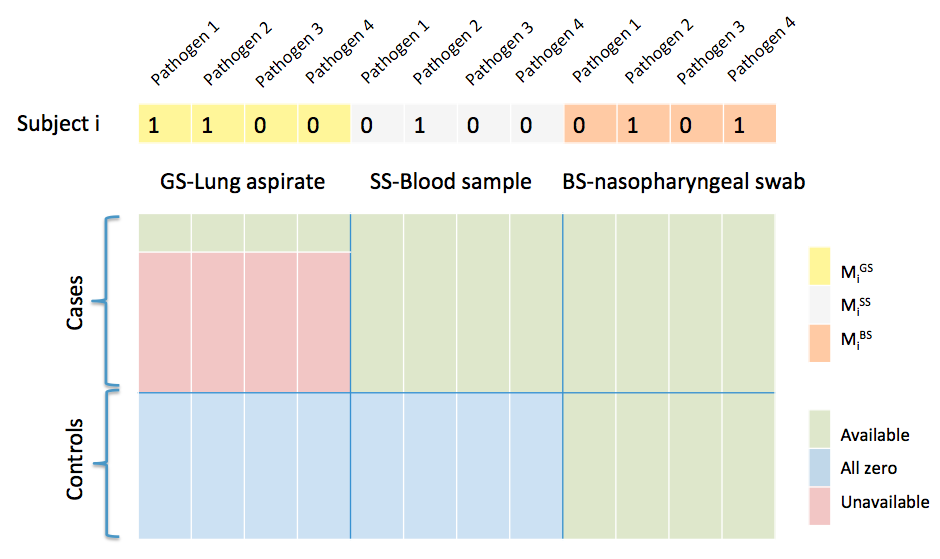
\includegraphics[scale=0.45]{DataDescription.png}
\captionof{figure}{{\bf Data Description}: }
\label{data}
\end{center}


\section{PERCH Data Analysis}
As what has been introduced in the first section of this paper, the PERCH study enrolled about 4200 children hospitalized for severe/very severe pneumonia and approximately 5300 controls randomly select from communities across $7$ sites around the world. To demonstrate the application of the LSC model for the analysis of PERCH study data, only the Kenya site data, where there is good availability of both BS and SS measurement data, is used so that the site-specific effect if not a concern. 


\section{Conclusion}


\bibliographystyle{plain}
\bibliography{draft_latentquadexp.bib}

\section*{Appendix}

\begin{table}[htbp]
\begin{adjustwidth}{-0.5in}{-1in}
\resizebox{0.7\textwidth}{!}{\begin{minipage}{\textwidth}
\caption{Summary of the True Parameter Values}
\label{tab: truepar}

\begin{tabular}{llllllllllllllll} 
\hline 
$\mu_1$ & $\mu_2$ & $\mu_3$ & $\pi_0$ & $\pi_1$ & $\pi_2$ & $\pi_3$ & TPR$^{(SS)}_1$ & TPR$^{(SS)}_2$ & TPR$^{(SS)}_3$ & TPR$^{(BS)}_1$ & TPR$^{(BS)}_2$ & TPR$^{(BS)}_3$ & FPR$^{(BS)}_1$ & FPR$^{(BS)}_2$ & FPR$^{(BS)}_3$ \\
\hline \\
$0.584$ & $0.289$ & $0.378$ & $0.10$ & $0.60$ & $0.25$ & $0.05$ & $0.05$ & $0.10$ & $0.10$ & $0.75$ & $0.80$ & $0.70$ & $0.50$ &  $0.50$ & $0.40$\\ \hline
\end{tabular}
\end{minipage}}
\end{adjustwidth}
\end{table}


\end{document}


%\begin{table}[htbp]
%\begin{adjustwidth}{-0.5in}{-1in}
%\resizebox{0.7\textwidth}{!}{\begin{minipage}{\textwidth}
%\caption{Summary of the model coefficients and standard error estimates}
%\label{tab: coef}
%
%\begin{tabular}{llllll|lllll} 
%\hline 
% \\
%\hline \\
%\end{tabular}
%\end{minipage}}
%\end{adjustwidth}
%\end{table}



















